\documentclass[10pt,twocolumn,letterpaper]{article}

\usepackage{wacv}
\usepackage{times}
\usepackage{epsfig}
\usepackage{graphicx}
\usepackage{caption}
\usepackage{subcaption}
\usepackage{amsmath}
\usepackage{amssymb}

% Include other packages here, before hyperref.

% If you comment hyperref and then uncomment it, you should delete
% egpaper.aux before re-running latex.  (Or just hit 'q' on the first latex
% run, let it finish, and you should be clear).
%\usepackage[pagebackref=true,breaklinks=true,letterpaper=true,colorlinks,bookmarks=false]{hyperref}

%\wacvfinalcopy % *** Uncomment this line for the final submission

\def\wacvPaperID{****} % *** Enter the wacv Paper ID here
\def\httilde{\mbox{\tt\raisebox{-.5ex}{\symbol{126}}}}

% Pages are numbered in submission mode, and unnumbered in camera-ready
\ifwacvfinal\pagestyle{empty}\fi
\setcounter{page}{1}
\begin{document}

%%%%%%%%% TITLE
\title{Urban Tribe}

%Authors at the same institution
\author{Yufei Wang \hspace{2cm}  Garrison Cottrell \\
University of California, San Diego\\
{\tt\small yuw176@ucsd.edu}
}
% Authors at different institutions
%\author{First Author \\
%Institution1\\
%{\tt\small firstauthor@i1.org}
%\and
%Second Author \\
%Institution2\\
%{\tt\small secondauthor@i2.org}
%}

\maketitle
\ifwacvfinal\thispagestyle{empty}\fi

%%%%%%%%% ABSTRACT
\begin{abstract}
We explore the use of pre-trained convolutional neural network features for social group recognition. A social group recognition framework is proposed. It takes in both individual and global features of group images, and shows promising results  for group recognition task which significantly outperform previous results. We verify the generalization ability and semantic information of pre-trained CNN features. We show the necessity of  fine-tuning in social group recognition, and this suggests a potential usage of pre-trained CNN features with adaptation for novel computer vision tasks. 

\end{abstract}

%%%%%%%%% BODY TEXT
\section{Introduction}

{I}{n} the past few years, there have been impressive progress in understanding semantic meaning of images, such as object recognition, scene recognition, and object detection. The power of Convolutional Neural Networks (CNNs) has is especially noticeable. However, studies in analysis of a group of people in images are still deficient. Current search algorithms fail to capture information of personal styles or social characteristics of groups of people, but retrieve images with similar global appearance \cite{urbantribe2}. The analysis of groups of people is difficult in that the group categories are semantically ambiguous, and have high intra-class variance.

Recognition of groups of people from a social perspective provides many potential applications.  With more accurate group searching results, more accurate recommendations can be made in social networks, and more relevant advertisement for particular groups of people benefits both consumers and sellers.

\cite{urbantribe} and \cite{urbantribe2} studied this problem of group recognition. They created an urban tribe dataset consisting of 11 categories, with about 100 labeled per class.  They proposed a group recognition pipeline. Rather than classifying isolated individuals in the group images, they focused on group features and models.

CNN architecture has been proved to achieve outstanding results in various computer vision tasks, and it's argued that deep architectures in CNN can capture visual features of different semantic level in the hidden units (\cite{Imagenet13}). Recently, features learnt for large scale recognition tasks with large amounts of training data have been used for new tasks, and the features outperform many conventional features in many tasks(\cite{Imagenet13}, \cite{decaf}). This verifies that generic visual features are obtained from pre-trained CNN model. 

\emph{this is what to modify later with results}
\textcolor{red} {The most frequently used pre-trained model was proposed in \cite{Imagenet} trained with ImageNet\footnote{http://image-net.org/challenges/LSVRC/2012/browse-synsets}. And the new tasks for which CNN features are used range from object recognition, scene recognition, to subcategory recognition. However, the objects or categories of these tasks are mainly covered in the 1000 ImageNet categories, and it is predictable that some features pre-trained on ImageNet are useful for the new tasks. Meanwhile, the social groups of individuals require semantic features of individual's style, which have little overlap with the 1000 ImageNet categories.}


%, and using the pre-trained features for social group recognition requires the network to find 
%such as object recognition on Caltech-101 dataset, Caltech-256 dataset (\cite{decaf}), Domain adaptation task on office dataset, subcategory recognition on Caltech-UCSD birds dataset, scene recognition on SUN-397 dataset


In this paper, we investigate the generalization ability of pre-trained CNN features to social group recognition.
We propose a CNN feature based architecture for social group recognition. Our model takes in both individual feature and global scene feature finetuned from CNN pre-trained weights. Our result shows a boost of performance from the previous group classification method provided by \cite{urbantribe2}. We show that both individual information and global scene information contribute to a social group's characteristics, and that different feature extraction schemes for individual and global information is necessary. We also show the role of adapting generic pre-trained CNN features to social group images with finetune. 

Further, we visualize the CNN features in different layers, and show a better semantic clustering with ascending layer, validating the feature composition of our framework. Finally, we analyze the properties of the social groups and the urban tribe dataset, showing that the representation our model achieves is in a high semantic level. 


\section{Related Work}
Convolutional Neural Networks(CNNs) with back-propogation were introduced around 1990's by \cite{lecun89}.  Since then, CNNs showed successful results on various computer vision tasks, such as hand-written digit classification (\cite{lecun98}), classification task on ImageNet dataset (\cite{Imagenet}). 

Recently, many researches show the ability of generalization of pre-trained CNN features on large dataset such as ImageNet. \cite{Imagenet13} shows excellent generalization of the pre-trained CNN features. They kept all the layers of ImageNet-trained model fixed except last softmax classifier, and achieved bets results on Caltech-101 and Caltech-256. \cite{decaf}  used different layers of pre-trained CNN network as features and trained simple classifiers such as SVM and Logistic Regression, and outperformed the state-of the-art on several vision challenges such as scene recognition and domain adaptation. 
GoogLeNet \footnote{http://www.image-net.org/challenges/LSVRC/2014/results} used improved CNN architecture pre-trained on ImageNet dataset, and won the the detection task of Large Scale Visual Recognition Challenge 2014 (ILSVRC2014). 

\cite{urbantribe2} created an urban tribe dataset consisting of 11 classes. The classes are defined from social group labels provided by Wikipedia. They selected the eight most popular categories from their list of subculture, and added three other classes corresponding to typical social venues  in addition. For each classes, images of groups of people are searched with different search engines, and a broad range of scenarios for each class are collected.   \cite{urbantribe} and \cite{urbantribe2} also provide a group description and several classification methods. Group description consists of person descriptors and global group descriptors: Six part of person is detected, and a set of predefined descriptors are computed for each part; Global descriptors use a both low level and high level descriptors to describe the context and group properties of the image. Two options of classification methods are provided: bag of parts-based classification and SVM-based classification.

Categorizing the social groups of individuals belongs to fine-grained classification task which recently draws more interest of the computer vision community. It aims at giving the fine-grained categories in a certain class. Fine-grained classification is more difficult than conventional classification tasks, because the categories are semantically as well as visually similar, and are even challenging for humans. The Fine-grained Challenge 2013 (FGComp) provided the data in several categories including aircraft, birds, cars, dogs, and shoes. \cite{finegrain} achieved the best result using classifier based on fisher vectors. However, CNN based methods using \cite{caffe} or \cite{decaf} gave not so good results, especially when the bounding box of test data is missing.

There is some research in analyzing social groups of people. \cite{groupstructure} showed the visual structure of a group helps understanding events. \cite{socialrelationship} showed social relationships modeling helps people recognition. \cite{happiest} used both local and global factors for group level expression analysis.




\section{Methods}
This section describes the urban tribe dataset and elaborates on the model architecture.

\subsection{Urban tribes dataset}
Urban tribes are groups of people who have similar visual appearances, personal style and ideals. The urban tribes dataset consists of 11 different categories: biker, country, goth, heavy-metal, hip-hop, hipster, raver, surfer, club, formal, casual/pub, with an average of 105 images from each category. 

Different from conventional visual classification problem, urban tribe categories are more ambiguous and subjective. Also, each class contains a broad range of scenarios. The high intra-class variation of the urban tribe dataset makes the classification task challenging. The urban tribe dataset also has some interesting properties. The number of people in each urban tribe image varies. Members in one tribe often have similar visual styles, including their clothes, accessories, and even demeanor. For example, surfers possibly carry surfboards, and the goth often have dark attire, makeup and hair. The environment they are in also contributes to each tribe characteristics: pictures of countries are more likely to be taken outdoor with grassland, while pictures of clubbers are often photographed in clubs with dim lightings. 

\subsection{Classification hierarchy}
%and and both the appearance of people and the environment they are in both contribute to the urban tribe characteristics.

To utilize the properties of urban tribes fully, our feature vector consists of both elements: individual features and environment features. For each feature type, we use similar extraction strategy. Individual features and environment features are hierarchically combined to form the final decision function.
The network hierarchy is shown in Figure~\ref{Flowchart}. 

For each group image, we represent the group $G$ as the combination of a set of people and the environment. To give the prediction of class $C$, the individual feature vectors and environment feature vectors are extracted separately.
 
For the individual feature vectors, first, individual person candidates are detected with a poselet based person detection algorithm. The person candidate images $H = \left\{H_{1}, H_{2}, ..., H_{p} \right\}$ are used as a whole instead of a set of body part bounding boxes. Each person candidate is resized to $256 \times 256$, and ten $227 \times 227$ patches $\left\{h_{ij}\right\}, i \in \left\{1,2,..,p\right\}, j=1,2,...,10$ are extracted using the same method as fine-tune image set generation. 

Each Individual image patch $h_{ij}$then passes through the Convolutional Neural Network for person images $\textup{CNN}_{Person}$, generating activations from the 6th and 7th hidden layer. The activations from 6th and 7th layer are both in 4096 dimensions. They are concatenated to form a 8192-dimensional vector $f_{ij}$, where $i \in \left\{1,2,..,p\right\}, j\in \left\{1,2,...,10\right\}$. 

The feature vectors are then fed into a multi-class $\textup{SVM}_{Person}$. We use LIBLINEAR\cite{liblinear} to train the SVM on individual patches, and to estimate probabilities for each category given individual patch $h_{ij}$: $\textup{Pr}_{ij}(C|h_{ij}), C \in \left\{1,2,..,c\right\}$, where $c$ is the number of classes in urban tribe dataset. The individual patches $h_{ij}$ in one group image are usually highly correlated. Therefore, in order to obtain a reliable probability estimate from the noisy yet correlated set of probabilities $\text{Pr}_{ij}$, a simple but effective average pooling is performed to $\textup{Pr}_{ij}$:
\begin{equation}
\textup{Pr}_{People}(C|H_{1}, ..., H_{p})=\frac{1}{10p}\sum_{i,j}\textup{Pr}_{i,j}(C|h_{ij})
\end{equation}
$\textup{Pr}_{People}(C|H_{1}, ..., H_{p})$ is the probability estimate of class $C$ given the set of people candidate images $H$. 

On the other hand, the entire environment in the scene image, denoted by $S$,  is directly utilized for probability estimation. The procedure to generate probability estimate of class $C$ given the environment as a whole $\textup{Pr}_{Scene}(C|S)$ is similar with that for $\textup{Pr}_{People}(C|H)$. The difference is that the input of Convolutional Network is $227\times227$ patches extracted from the entire scene image, and the fine-tuned Convolutional network: $\textup{CNN}_{Scene}$ and SVM: $\textup{SVM}_{Scene}$ are trained with the training set of entire scene images. Several different strategies to extract patches from scene images and corresponding Convolutional Neural Network architectures are explained in Section~\ref{sectioncnn}.

Therefore, the probability estimate of a class $C$ given observation of scene $S$ is:
\begin{equation}
\textup{Pr}_{Scene}(C|S)=\frac{1}{K}\sum_{k=1}^{K}\textup{Pr}_{k}(C|s_{k})
\end{equation}
where $K$ is the number of scene patches extracted from one group image, and this number varies with different patch extraction strategies. $s_{k}$ is the $k$th scene patches. $\textup{Pr}_{k}(C|s_{k})$ is the probability for class $C$ given $k$th scene patch. Average pooling is still used here, because the assumption of high correlation in patches holds. 

Now we have the estimates of two kinds of conditional probability $\textup{Pr}_{People}(C|H)$ and $\textup{Pr}_{Scene}(C|S)$. We make a strong assumption that the two types of features are independent, and that the prior probability distribution of the urban tribes $\textup{Pr}(C)$ is a uniform distribution. The classification problem can be expressed as maximizing the objective function:
\begin{equation}
L = \textup{arg max}_{i=1,...,c}\textup{Pr}(C=i|G)
\end{equation}
where
\begin{equation}
\begin{split}
 \textup{Pr}(C=i|G)& =\textup{Pr}(C=i|H, S) \\
  & = \frac{\textup{Pr}_{People}(C=i|H_{1},...,H_{p}) \cdot \textup{Pr}_{Scene}(C=i|S)}{\textup{Pr}(C=i)} \\
  & \propto \textup{Pr}_{People}(C=i|H_{1},...,H_{p}) \cdot \textup{Pr}_{Scene}(C=i|S)
\end{split}
\end{equation}
and $L$ is the predicted label for the group image. 


\begin{figure*}[t]
\begin{center}
%\fbox{\rule{0pt}{2in} \rule{0.9\linewidth}{0pt}}
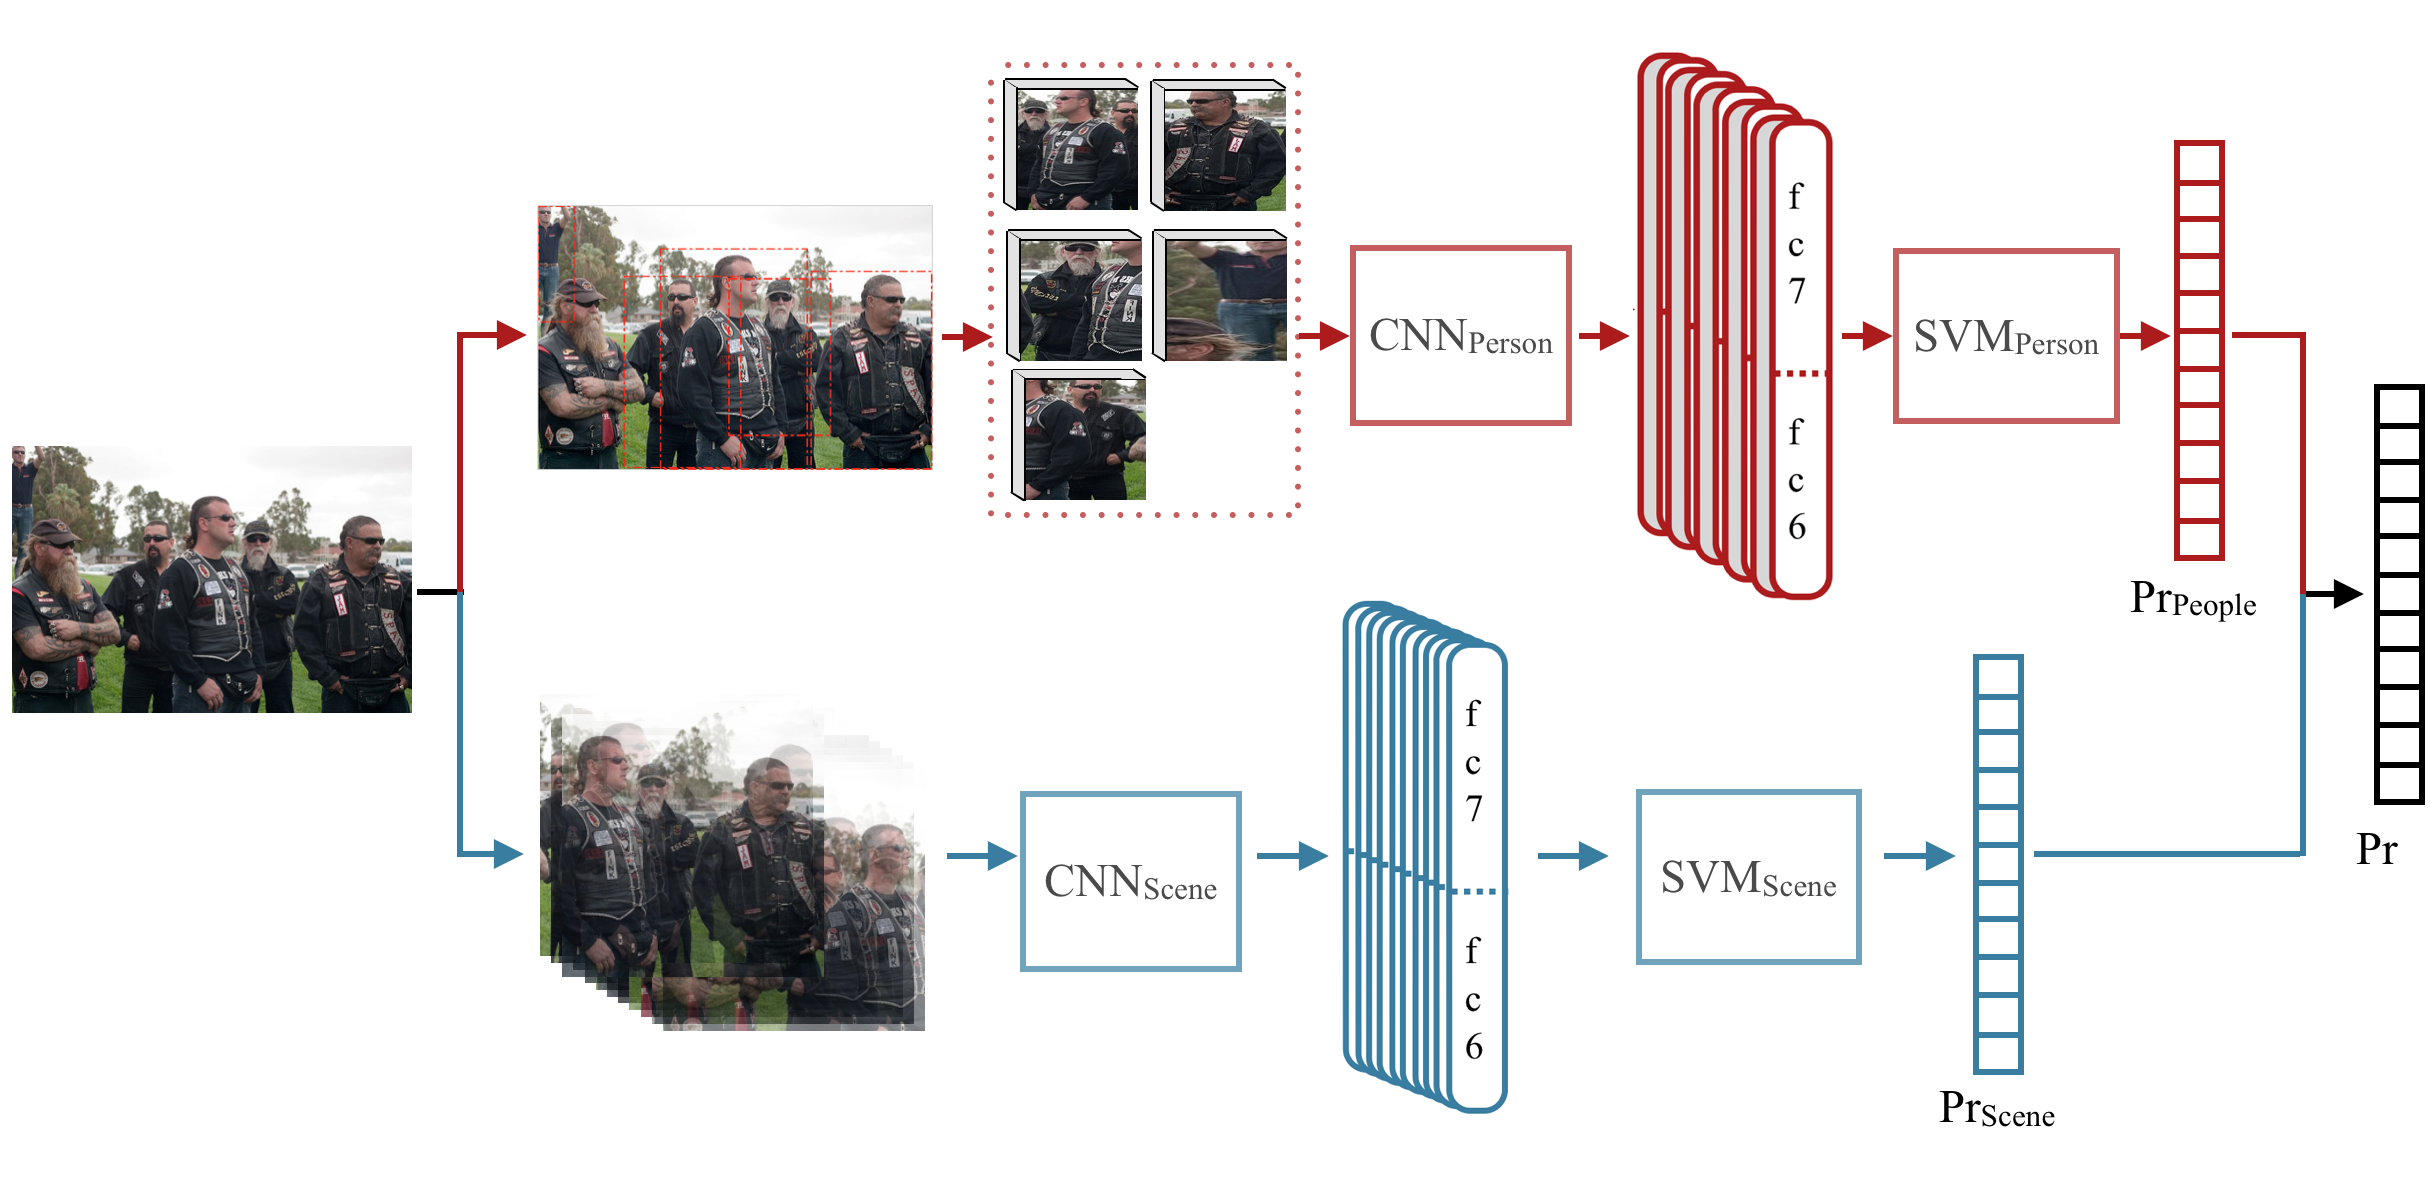
\includegraphics[width=0.8\linewidth]{flowchart2}
\end{center}
   \caption{Architecture of classification algorithm using $\textup{Nets}_{SDense}$. The upper half estimates the probability given people candidate images, and the lower half estimates the probability given the entire scene. Dense crop $\textup{CNN}_{Scene}$ and distorted crop $\textup{CNN}_{Person}$ are used.}
\label{Flowchart}
\end{figure*}



\subsection{Convolutional network feature extraction}
\label{sectioncnn}
It is shown in many experiments that a set of weights of convolutional network trained from ImageNet can generate a set of generic visual features.

Following \cite{caffe}'s work, we use the network framework called Caffe. The network architecture is described in \cite{Imagenet}, which won the ImageNet Large Scale Visual Recognition Challenge 2012. We take the activations from the 6th and 7th hidden layer of the convolutional neural network, which are two fully connected layers before the class prediction layer. We also take the activations from 6th or 7th layer alone as comparison. We choose these two layers, because as the layers ascend, the features extracted show increasing invariance and semantic meaning. 

We use the pre-trained set of weights of the network released by Caffe as the initial parameters of our network. The pre-trained model was trained on Imagenet ILSVRC-2012, and all images are first resized to $256\times256$ before they can be used as inputs to the network.

\subsubsection{Pre-processing of the dataset}
\label{sectioncropping}
The urban tribe dataset is a relatively small dataset, and both people candidate crops and scene images are of various resolution. Our convolutional neural networks requires constant input image size of $227\times227$, so pre-processing of the dataset is necessary. 

There are several strategies to make one image compatible with the CNN:

\begin{enumerate}
\item As in \cite{Imagenet}, resize the image to a fixed resolution of $256\times256$, and crop five $227 \times 227$ patches (from four corner and the center) and their horizontal reflections to generate ten patches from one single image. This way, the aspect ratio of the original images are lost, but for each crop, the portion it takes from the original image is fixed, so that the amount of information all the crops have is relatively stable.
\item Keep the aspect ratio of the original image, resize the shorter side to 256, and then crop five $227 \times 227$ patches and their horizontal reflections as mentioned. This method avoids distortion of the image and objects in it, but the crops will possibly lose much information when the aspect ratio of the original image is far away from 1.
\item Keep the aspect ratio of the original image, resize the shorter side to 256, and then densely crop multiple $227 \times 227$ patches and their horizontal reflections. This way, the information of original image is kept by dense cropping process, and the distortion is avoided. The number of crops attained with this method is larger than the previous two methods.
\end{enumerate}

\subsubsection{Network Finetune}
Although the pre-trained network from \cite{caffe} can already generalize well to many datasets, the urban tribe dataset has its unique property. It emphasizes certain visual features such as clothes, while pays less attention to other visual features. Also, it emphasizes style of the object rather than distinct category. To rearrange the importance of different features and adjust the features to adapt to urban tribe dataset, the network can be finetuned. 

The dataset used for finetune is the same set used for future training. The input patches of the Convolutional network is of size $227 \times 227$. The initial Convolutional network has 1000 outputs in final layer, corresponding to 1000 class-wise probability predictions. In our finetune process, the last layer is replaced by 11 probability prediction outputs, and the initial weights of the last layer connection are initialized to have zero mean gaussian distribution. Back propagation is used, and the learning rate is set to be small so that the fine-tune process adapts the extracted features to urban tribe dataset while preserving the initial property in general: the initial learning rate used for pretraining is 0.01; We set the initial finetune learning rate of the parameters except for the last layer as 0.001, and keep the initial learning rate for last layer 0.01, because the last layer is not pre-trained.


\subsubsection{Network modification}
The side effect of dense cropping technique in Section~\ref{sectioncropping} is that there is a boost in the number of input crops, and the speed of feature extraction is largely slowed down. 

We apply a trick to speed up the process. In a convolutional neural network, a fully connected layer can be viewed as a convolutional layer with $1\times1$ sized kernels. Therefore, in our CNN architecture, we can substitute convolutional layers for fully connected layers of 6th and 7th layer. For example, the input of 7th layer is 4096-dimensional feature, and the output is 4096-dimensional feature. The layer has $4096\times 4096$ connections. We can view the connections as $4096\times 4096$ convolutional filters with size $1\times1$. For one input image of size $227\times227$, the output of the 7th layer is 4096 feature maps of size $1\times1$, while for one input image of arbitrary size (larger than $227\times227$), the output of the 7th convolutional layer is 4096 feature maps of larger size, each 4096-dimensional element corresponds to one $227\times227$ cropping of the input image. Now the modified network can take images with arbitrary size (larger than $227\times227$) as input, and extract patch features much more efficiently. 

\subsubsection{Choices of network combination}
\label{sectionmethods}
Scene images and individual images have different properties, and need different strategies of pre-processing and separate fine-tuning. For scene network $\textup{CNN}_{Scene}$ and scene images, due to the small size of the dataset, we use the dense cropping technique to increase the dataset. Only the center crops of each original group image and their mirrors are used for finetune.  For person network $\textup{CNN}_{Person}$ and corresponding input, we use the first cropping technique, because the subimages have normally long height and short width, and the second and third strategies using squared crops of a person image will lose much information, no matter which location we choose to crop them; whereas the first method ensure each crop keeps the essential features for classification. Finetuning of $\textup{CNN}_{Person}$ uses center crops and their mirrors of person candidate images. 

The combination of dense crop $\textup{CNN}_{Scene}$ and distorted crop $\textup{CNN}_{Person}$ are denoted as $\textup{Nets}_{SDense}$.

We also construct other combination of networks for comparison:
\begin{enumerate}
\item $\textup{Nets}_{NoTune}$: Directly use the pre-trained network by \cite{caffe} for both scenes and persons, and use the first cropping technique (distorted crops) as input patches for both networks. This choice of cropping strategy is in consistent with the way the network is pre-trained.
\item $\textup{Nets}_{SSparse}$: Use the second cropping strategy for scene features, and the first cropping strategy for person features. Finetune procedure is the same as $\textup{Nets}_{SDense}$.
\item $\textup{Nets}_{SDistort}$: Use the first cropping strategy for both scene features and person features. Training set for finetune procedure is the center crops and their mirrors of scene/person images.
\end{enumerate}


\section{Experiments and Results}
In this section, the performance of the proposed classification scheme is evaluated and analyzed. In the experiments, six rounds of 5-fold cross validation are performed, therefore we have 30 training experiments in total. Dataset is partitioned into 5 equal sized subsets, containing one-fifth of the data points from each category. One of the subsets is used as test set, and the remained 4 subsets are used as training data. In the finetune procedure, there are 6000 training iterations, and learning rate is decreased by ten times after each 1000 iterations.


\subsection{Urban tribe classification performance}

\begin{table*}[!t]
\centering
    \caption{Performance of different approaches using different information. }
    \label{table1}
    \begin{tabular}{l|l|l|l|l}
    \hline
    Accuracy (\%)                                          & Individual candidate & People & Entire scene & People+Scene \\ \hline

$\textup{Nets}_{SDistort}$   with concatenated features               & $39.99\pm0.30$                    & $64.09\pm0.63$      & $62.77\pm0.52$            & $69.28\pm0.50$            \\ \hline
    $\textup{Nets}_{SDense}$ with fc7 features & $47.07 \pm0.30$ & $67.09 \pm 0.52$      & $65.05 \pm0.42$            & $70.74\pm0.47$      \\ \hline
     $\textup{Nets}_{SDense}$ with fc6 features & $45.84 \pm0.34$ & $66.20 \pm 0.46$      & $67.08 \pm0.51$            & $70.43\pm0.46$      \\ \hline
     $\textup{Nets}_{SDense}$ with concatenated features     &  $\mathbf{47.10 \pm0.34}$ & $\mathbf{67.29 \pm 0.50}$      & $\mathbf{67.26 \pm0.50}$            & $71.22\pm0.46$      \\ \hline
    $\textup{Nets}_{SSparse}$ with concatenated features               & $\mathbf{47.10 \pm0.34}$                    &$\mathbf{67.29  \pm 0.50}$        & $66.81\pm0.42$            & $\mathbf{71.23\pm0.49}$            \\ \hline
    $\textup{Nets}_{SDistort}$ with concatenated features               &  $\mathbf{47.10 \pm0.34}$          &$\mathbf{67.29 \pm 0.50}$       & $65.35\pm0.37$            & $71.15\pm0.50$            \\ \hline
    $SVM_{8}$\cite{urbantribe2} & - & - & - & $46$(std: $2$)  \\ \hline


    \end{tabular}
\end{table*}
\begin{figure}[!t]
\begin{center}
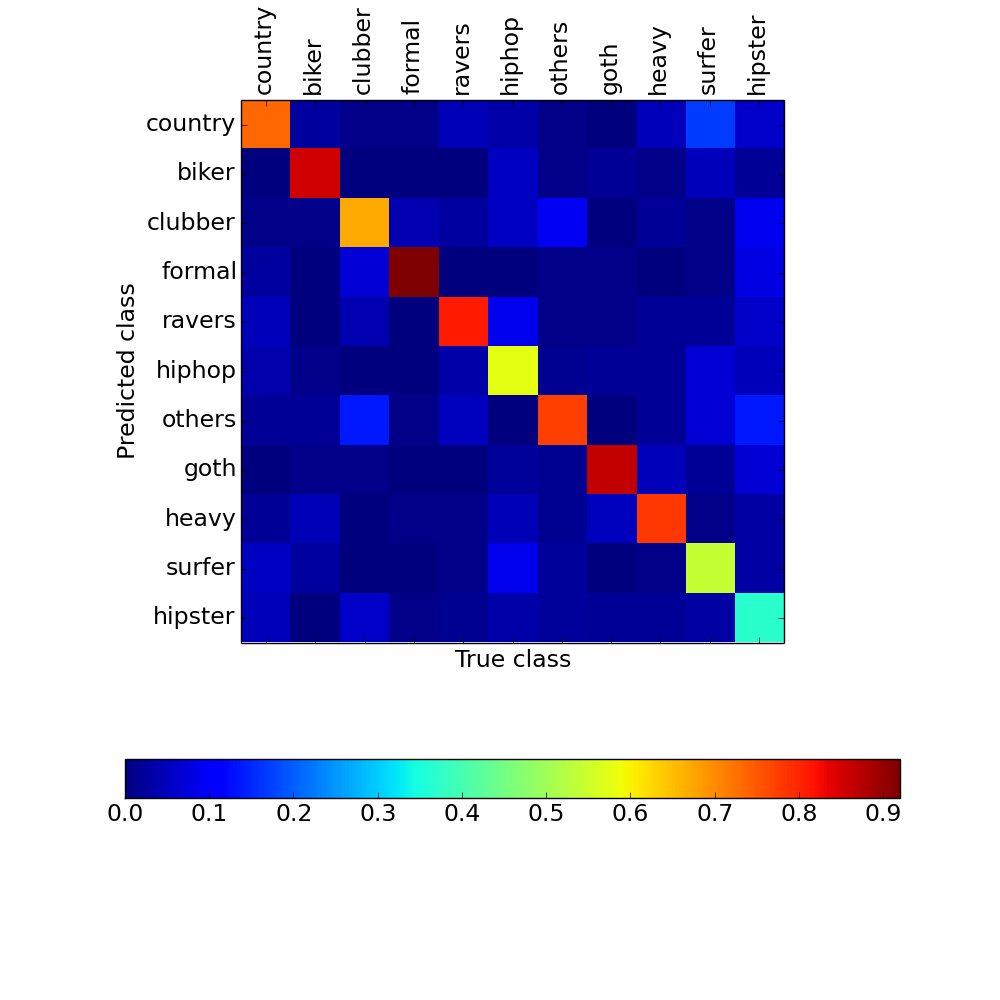
\includegraphics[width=0.8\linewidth]{confusion.png}
\end{center}
\caption{Confusion matrix for classification results with  $\textup{Nets}_{SDense}$,  using people and scene features.}
\label{confusion}
\end{figure}


Table~\ref{table1} shows the comparison of performance using different approaches. The 30 segmentations of datasets are used for all the approaches tested in this section, and 30 test results are averaged for each approach. The standard error is shown with the accuracy in Table~\ref{table1}. We also compare our result with the result achieved by \cite{urbantribe2} using their best model. The advantage of CNN pre-trained features is obvious. 

The confusion matrix is shown in Figure~\ref{confusion} for $\textup{Nets}_{SDense}$, and all the 30 training experiments are averaged. We can observe there is a obvious difference of difficulty of different categories. Class \emph{formal} has accuracy as high as about 90\%, while class hipster is the most difficult class, having less than 60\% accuracy.

%\subsubsection{Necessity of people and scene features}
Comparing the result of using different features in the same approach shows the necessity of every step of our architecture. In results using  $\textup{Nets}_{SDense}$ with concatenated features, average accuracy for each individual person candidate is low as 47.10\%. Average pooling of individual candidate probability estimates produces a large accuracy increase of about 20\%. Accuracy using the entire scene only results in 67.26\% accuracy. Combining probabilities $\textup{Pr}_{People}(C|H_{1}, ..., H_{p})$ and $\textup{Pr}_{Scene}(C|S)$ achieves accuracy as high as 71.22\%, which verifies the complementary role of people candidate feature and environment feature in a group image. 

%\subsubsection{The role of feature concatenation and finetune}
We also compare vertically the accuracy of different approaches, to show the role of  network feature concatenation. Using only 7th layer or 6th layer activation from the networks $\textup{Nets}_{SDense}$ produces decent results, showing both layers' activations can generate high semantic features. Concatenating both layers' activations increases the accuracy by 0.5\%, indicating the slight information loss of the 7th fully connected layer. 

To see the role of finetuning, we can compare the result of $\textup{Nets}_{NoTune}$  and $\textup{Nets}_{SDistort}$. These two approaches both use resizing that causes distortion, and they only vary in finetune procedure. There is a large performance improvement with finetune, both for person features and scene features. This shows the benefit of adapting existing generic Convolutional Network to specific dataset. 

%Another interesting effect of fine-tune is the decrease of variance. Comparing to the result of $\textup{Nets}_{NoTune}$, fine-tuned networks $\textup{Nets}_{SDistort}$ yield a more stable result for both people features and scene features.

%\subsubsection{Comparison between different patch extraction strategies}
$\textup{Nets}_{SDistort}$, $\textup{Nets}_{SSparse}$, and $\textup{Nets}_{SDense}$ use different patch extraction strategies. Note that we use the same distorted patch extraction method for person images, as mentioned in Section~\ref{sectionmethods}, while we use three different methods for scene images. The results for scene images show the advantage of keeping the aspect ratio of scene images, and the slight advantage of using dense crops. However, the final results with People+Scene for the three methods don't have significant differences, this is due to the combination with people information. 

%The last three rows of Table~\ref{table1} indicate some interesting features of different patch extraction methods. 
%The entire scene accuracy of $\textup{Nets}_{SSparse}$, and $\textup{Nets}_{SDense}$ is more than 1.5\% higher than $\textup{Nets}_{SDistort}$, which verifies that preserving the aspect ratio of scene images is better than using distorted patches. 

%The overall accuracy of $\textup{Nets}_{SDense}$ is about 0.3\% higher than $\textup{Nets}_{SSparse}$, showing that densely extracting patches is useful. Interestingly, accuracy using only scene network $\textup{CNN}_{Scene}$ shows that $\textup{Nets}_{SDense}$ performs more than 0.3\% worse than $\textup{Nets}_{SSparse}$. This is due to the complementary property of people features and scene features.  Dense patches of scene images have more redundant information than sparse patches, thus reducing the performance of scene patches. However, the dense patches 'soften` the probability estimate $\textup{Pr}_{Scene}(C|S)$, making the judgement less confident. When scene information is combined with people features $\textup{Pr}_{People}(C|H)$, the advantage of the 'softening' effect appears: for $\textup{Nets}_{SDense}$, the wrong judgement made from scene information are more likely to be corrected by people information. This leads to a overall performance improvement of $\textup{Nets}_{SDense}$ despite the performance drop with scene information alone.

\subsection{Convolutional Network feature analysis}
\textbf{Yufei: Is this section necessary?}
We use t-distributed stochastic neighbor embedding technique \cite{tsne} to visualize the power of different layers' features in convolutional network. Two dimensional embedding of the high dimensional CNN feature space is extracted, and we plot the data as 2-d points with different colors indicating different classes they belong to. Powerful features will pull data of different semantic classes more apart.

We randomly choose one training-test partition and corresponding fine-tuned network parameters, and to avoid overfitting effect, we examine the test set of $\textup{Nets}_{SDense}$ approach. In Figure~\ref{tsne}, each data is plotted as a dot in each figure. The three columns correspond to data separation in first layer, fourth layer and seventh layer respectively. The first row visualizes features of all test data in scene CNN $\textup{CNN}_{Scene}$, and second row picks three classes from the first row. The third row is features of $\textup{CNN}_{Person}$, and the three classes are picked for the last row. The three classes chosen in second and last row is (goth:red, heavy:green, surfer:blue).

In both $\textup{CNN}_{Scene}$ and $\textup{CNN}_{Person}$, there is a clear trend of class separation. As the layer ascends, , the data from same class are more concentrate, and inter-class distance are larger. The selected three classes show the trend more clearly: they essentially form three clusters in the seventh layer. 
As shown in the second and last rows, person data is more challenging: The semantic classes are not as separate as with the scene features. 


%Especially, patches extracted from same image are very close to each other in the seventh layer. To see the trend more clearly, we randomly choose three classes (goth:red, heavy:green, surfer:blue) and plot them in the second row. The data becomes more concentrate within the same class while more separate with different class when the layer ascends. In the last layer, the three classes has essentially formed three clusters and can be roughly separated by simple classifier. Then, we proceed to examine the features of person network $\textup{CNN}_{Person}$. Person data is more challenging, and $\textup{CNN}_{Person}$ is expected to be less powerful. This is verified in the last two rows from figure~\ref{tsne}. We choose the same training-test dataset separation as in scene feature visualization, and for each person image, only center crop is plotted. The same trend occurs with the ascending layers, whereas the semantic classes are not as separate as with the scene features. Looking into the visualization of seventh layer (Second row third column), we can see three batches of dots labeled heavy far away from the 'heavy' cluster. The three clusters correspond to three urban tribe images, and the final classification results of the three images by the algorithm $\textup{Nets}_{SDense}$ are goth, goth, and hiphop respectively. All the three images are misclassified, and this validates the feature visualization result.When comparing the seventh layer features from $\textup{CNN}_{Person}$ and $\textup{CNN}_{Scene}$, we can observe the complementarity of the two types of features, and the necessity of combining them. Note that the color map is the same in both feature types. For some classes, scene features give a more powerful description; While for other classes, person feature map clusters the data more, for example the green points standing for bikers are better described in person CNN features. This is probably because bikers in many scene images have uniform clothing, which is better captured by person CNN features. 

\begin{figure}[!t]
\begin{center}
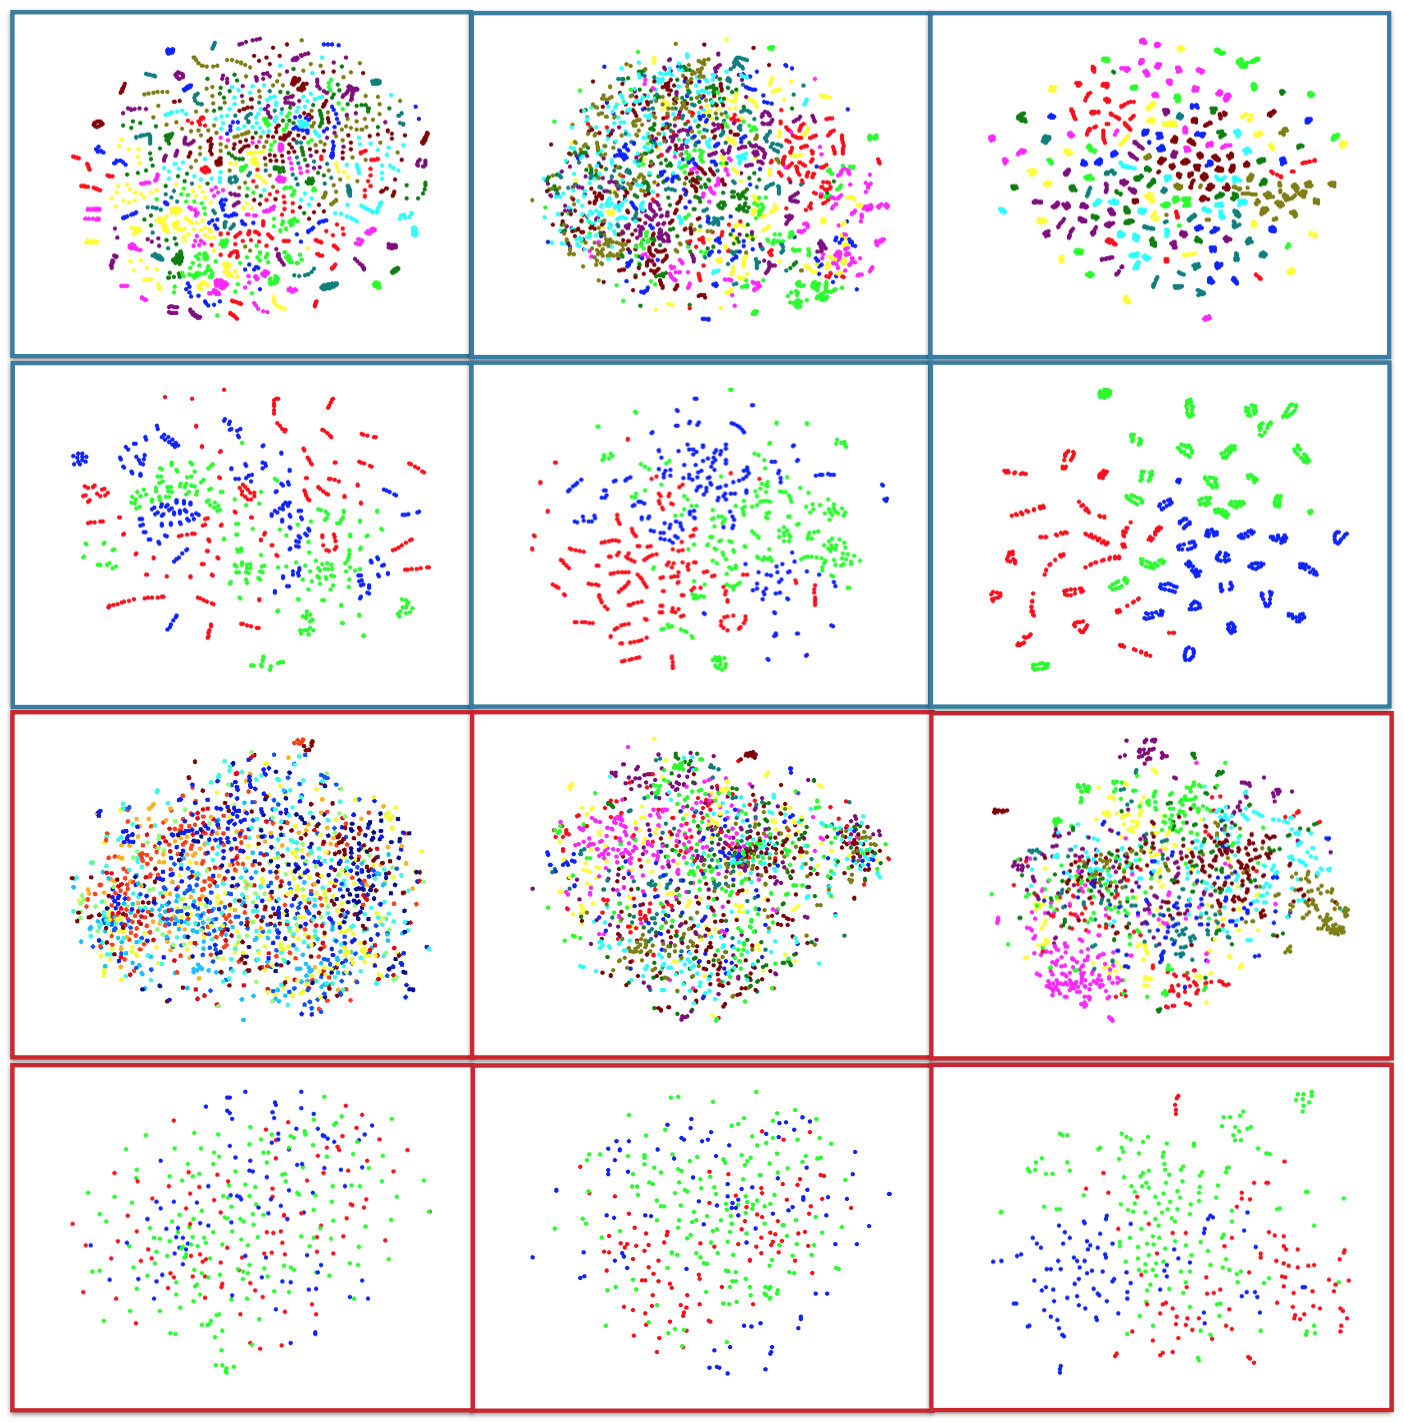
\includegraphics[width=0.8\linewidth]{tsne}
\end{center}
\caption{Feature visualization of  $\textup{Nets}_{SDense}$: $\textup{CNN}_{Scene}$ (first two rows) and $\textup{CNN}_{Person}$(second two rows). Rows: first: all scene images; second: all data from goth/heavy/surfer urban tribes; third: all test person images; fourth: all test data from goth/heavy/surfer urban tribes. Columns:  first: first convolutional layer; second: fourth convolutional layer; third: seventh fully convolutional layer}
\label{tsne}
\end{figure}

\subsection{Urban tribe classes vs. Imagenet classes }
It's recently being acknowledged that CNN pre-trained features are generic and can be used for new tasks. In this section we check the relationship between the new tasks and original Imagenet task, using the urban tribe dataset,which gives us some insight about the features extracted from pre-trained network.

The urban tribe dataset contains groups of people, and the important features for categorization are mainly human related features, such as attire, make up, posture and expressions. However, the ILSVRC dataset used for pretraining contains few images of humans. Instead of examining the output of the layers directly, we try to find the relationship between the 1000 classes in ILSVRC dataset and the classes in two image sets: urban tribe dataset, and person candidate images extracted from urban tribe dataset.

We use the parameters of pre-trained CNN network as our feature extraction model, and train a softmax layer  
on top of its 7th layer to predict the probabilities of one input image(either scene image or person candidate image) being in certain urban-tribe class $\textup{Pr}(l_{urban})$, where $l_{urban} $pre-trained is the 11 urban tribe categories. The output layer is trained for 3000 training iterations. We can also use the output of the pre-trained CNN network to predict probabilities of one input image being in certain Imagenet category, denoted as $\textup{Pr}(l_{Imagenet})$, where $l_{Imagenet}$ is the 1000 Imagenet categories. We use one round of 5-fold cross validation, and use all the images in urban tribe dataset for analysis.

We first check the relationshape of $\textup{Pr}(l_{urban})$ and $\textup{Pr}(l_{Imagenet})$ of person candidate images. We calculate the correlation coefficient of $\textup{Pr}(l_{urban})$ and $\textup{Pr}(l_{Imagenet})$ for all 1000 Imagenet classes, denoted as $R(\textup{Pr}(l_{urban}), \textup{Pr}(l_{Imagenet}))$. We also calculate the 1000 mutual information of the predicted score of urban tribe and Imagenet (where predicted score is 1 if the predicted label is the category being tested, 0 otherwise), denoted as $I(l_{urban}, l_{Imagenet})$. 

In Figure~\ref{correlation_muti}, we choose two urban classes: \emph{biker} and \emph{hipster}, and plot the correlation coefficient $R$ and mutual information $I$.The first row shows the result of \emph{biker}, and second row \emph{hipster}. For \emph{biker}, there are several impulses in correlation plot, and one significant impulse in mutual information plot. \emph{whiptail lizard} has high correlation with \emph{biker}. Meanwhile, for \emph{hipster}, which is the most difficult class, the correlation coefficient and mutual information are both low for all Imagenet classes.

To confirm the correlation,we use $\textup{Pr}(l_{Imagenet})$ directly as features, substituting the concatenated fc7fc6 features, and use the $\textup{Nets}_{SDistort}$ approach for classification. The accuracy is 52.68\%. This decent result indicates the relationship between $l_{urban}$ and $l_{Imagenet}$.
Then, we check $l_{Imagenet}$ with highest correlation coefficients with $l_{urban}$. In Figure~\ref{features}, we choose four $l_{urban}$: \emph{formal}, \emph{ravers}, \emph{goth}, \emph{hipster}, and choose some examples of person candidate images that have both high $\textup{Pr}(l_{Imagenet})$ and high  $\textup{Pr}(l_{urban})$. We also show examples of the images in $l_{Imagenet}$. We can see some of the shared features between corresponding person images and Imagenet images, for example, similar shape for women tops and stingrays (Figure~\ref{feature2}). 

There is a correlation between class-wise accuracy of predicted $l_{urban}$ and the degree of relationship between predicted $\textup{Pr}(l_{urban})$ and $\textup{Pr}(l_{Imagenet})$, as shown in Figure~\ref{accuracy_correlation_mutu}. Class-wise accuracy is calculated for person candidate images(Figure~\ref{sb1}, \ref{sb2}) or scene images(Figure~\ref{sb3}, \ref{sb4}). For each $l_{urban}$, the maximum correlation/mutual information over 1000 Imagenet classes are used to indicate the degree of its relationship with $l_{Imagenet}$.

The correlation between Imagenet class and urban tribe class and its relationship with class-wise recognition rate may indicate that \textcolor{red} {the ``generic" features extracted by pre-trained CNN networks are not so generic. The network is trained to separate the Imagenet classes most, and if we use the features for a new classification task, the performance of the task is related to how well the new classes can be ``mapped" to the Imagenet classes. }



\begin{figure}[!t]
\begin{center}
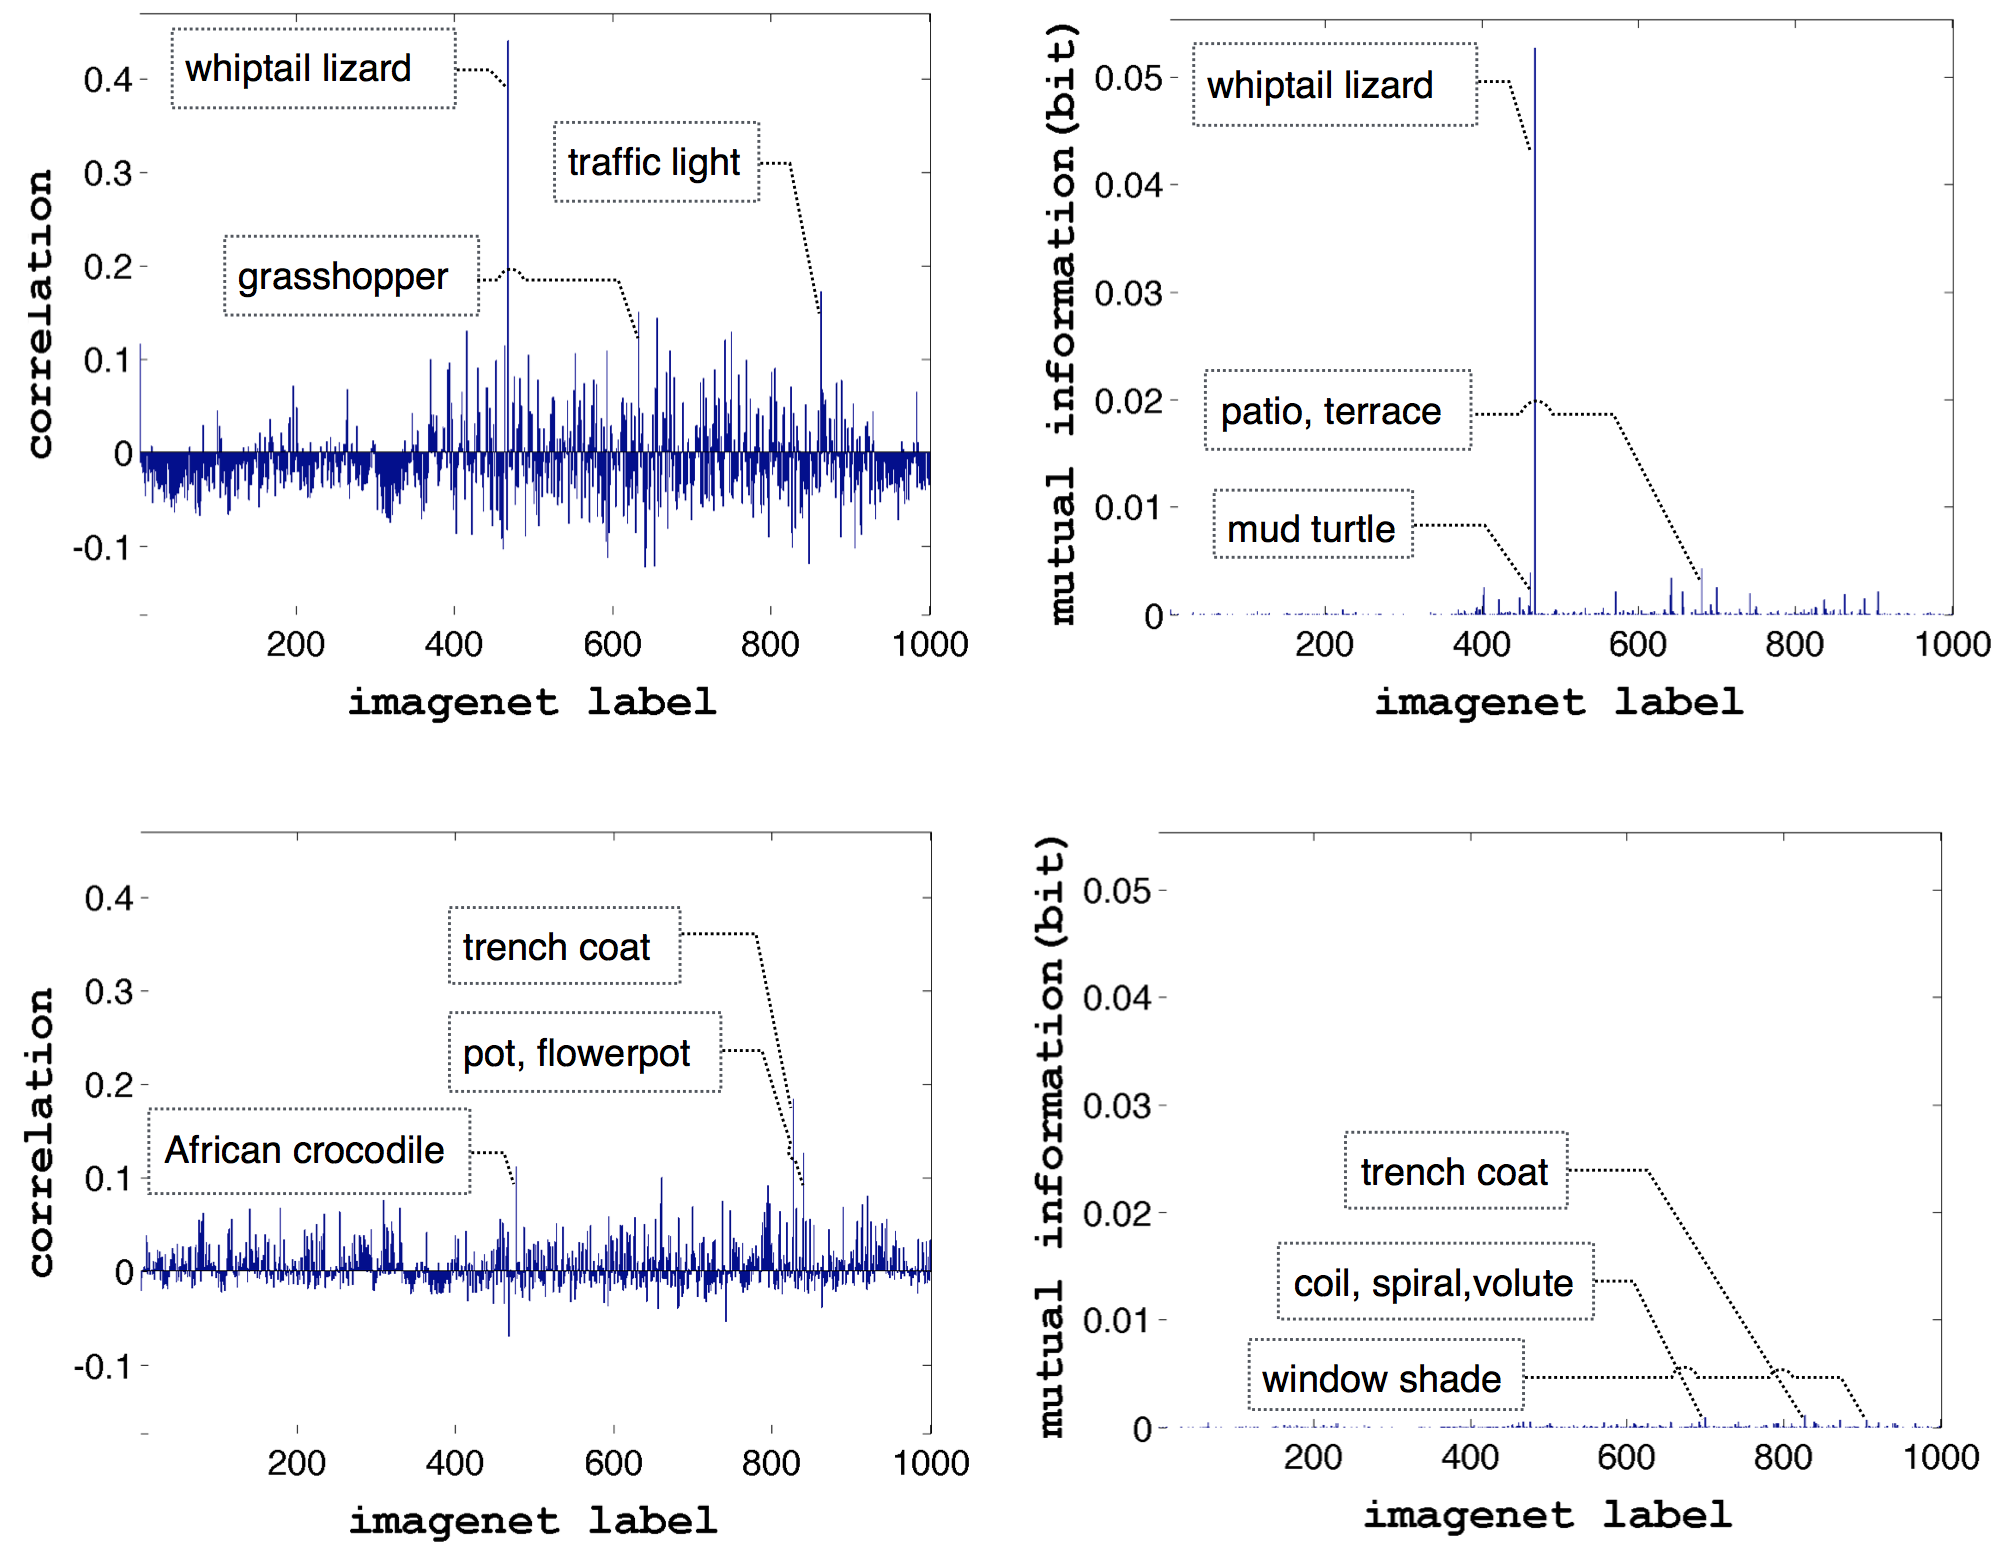
\includegraphics[width=1\linewidth]{correlation}
\end{center}
\caption{Correlation and mutual information of $l_{urban}$ and 1000 $l_{Imagenet}$. The first row is for $l_{urban}$=Biker. The second row is for $I_{urban}$=Hipster. Top three Imagenet classes are marked. }
\label{correlation_muti}
\end{figure}

\begin{figure*}[!t]
\begin{center}
        \begin{subfigure}[b]{0.2\textwidth}
                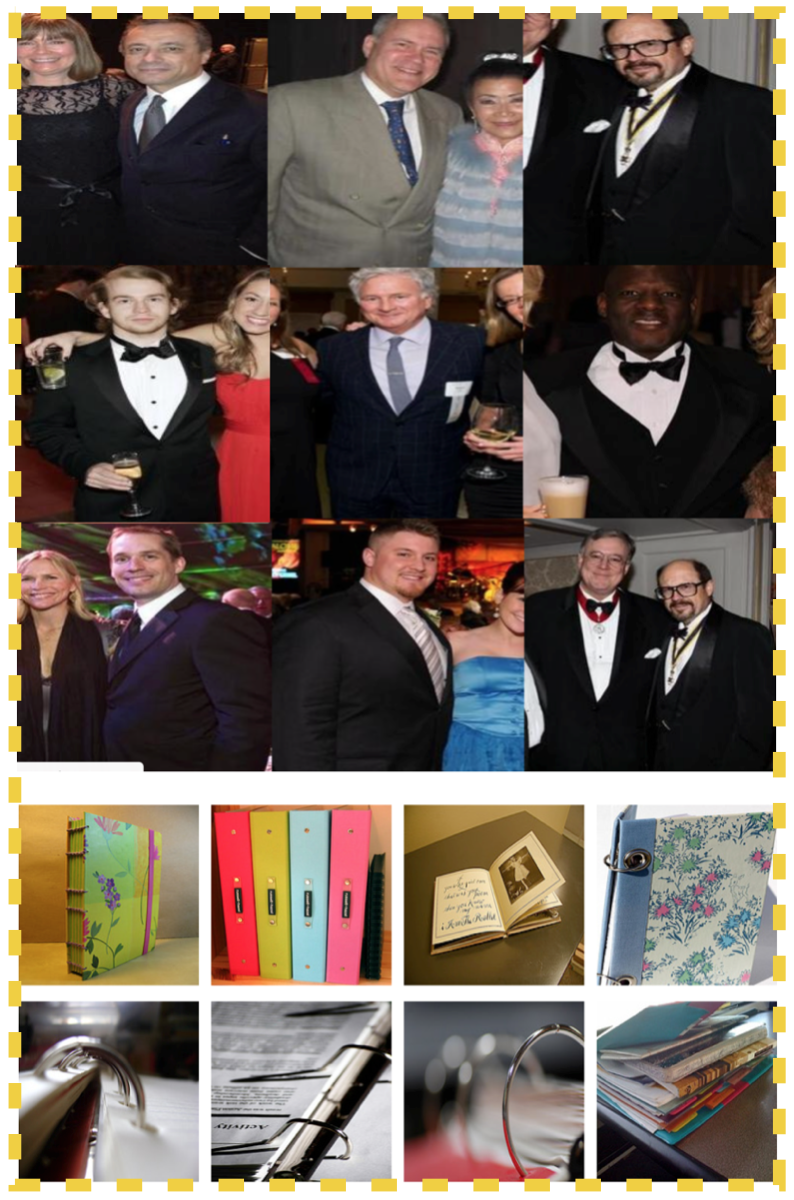
\includegraphics[width=\textwidth]{feature1}
                \caption{Formal - Binder}
                \label{feature1}
        \end{subfigure}
                \begin{subfigure}[b]{0.2\textwidth}
                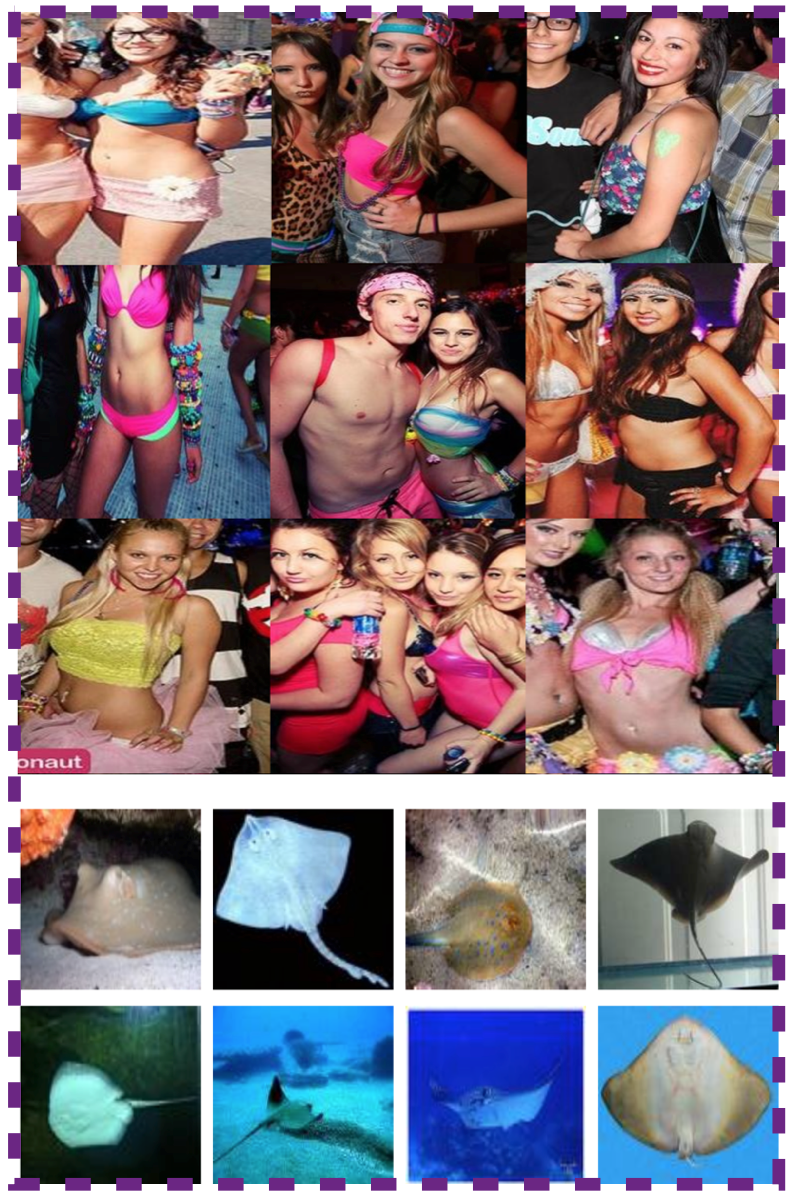
\includegraphics[width=\textwidth]{feature2}
                \caption{Ravers - Stingray}
                \label{feature2}
        \end{subfigure}
                \begin{subfigure}[b]{0.2\textwidth}
                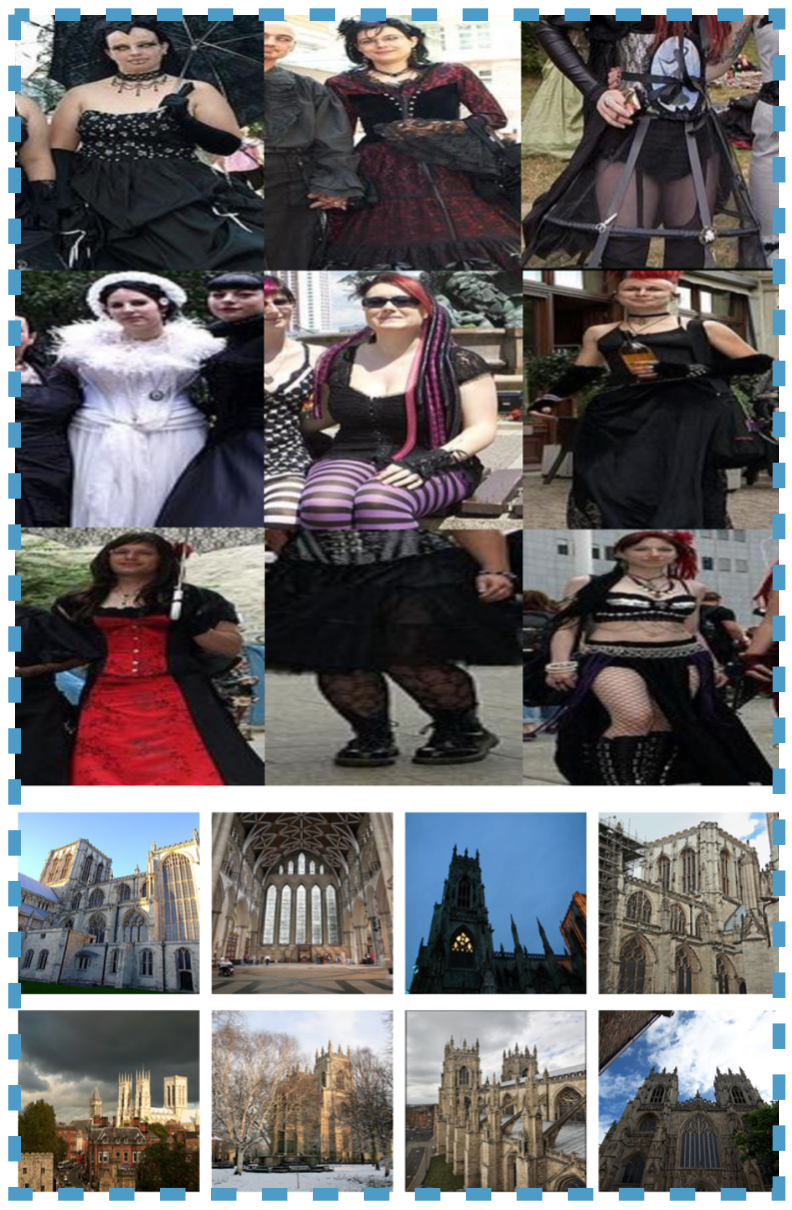
\includegraphics[width=\textwidth]{feature3}
                \caption{Goth - Church}
                \label{feature3}
        \end{subfigure}
                \begin{subfigure}[b]{0.2\textwidth}
                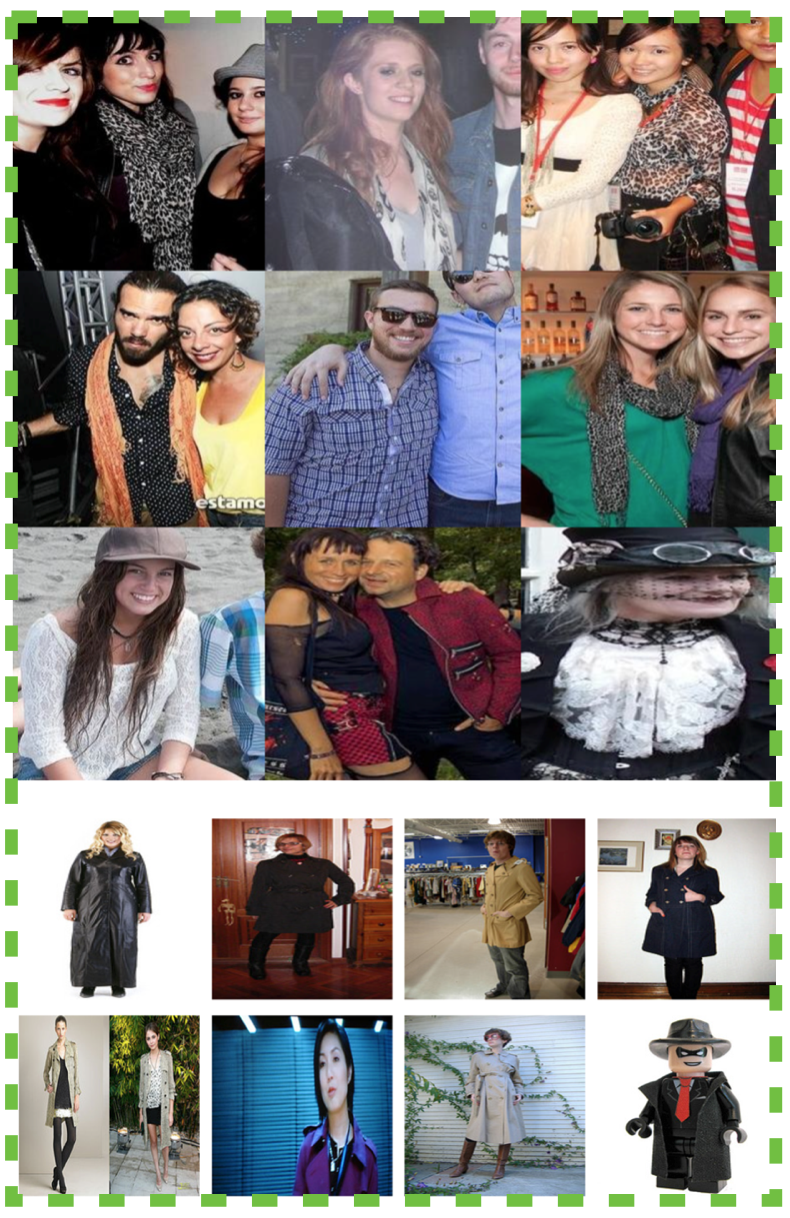
\includegraphics[width=\textwidth]{feature4}
                \caption{Hipster - Trench coat}
                \label{feature4}
        \end{subfigure}
\end{center}
\caption{selected urban tribe classes and the corresponding highest correlation $l_{Imagenet}$. Upper nine images: person candidate images with high $\textup{Pr}(l_{Imagenet})$ and high  $\textup{Pr}(l_{urban})$. Lower eight images: example of images in $l_{Imagenet}$.}
\label{features}
\end{figure*}

\begin{figure*}[!t]
\begin{center}
        \begin{subfigure}[b]{0.23\textwidth}
                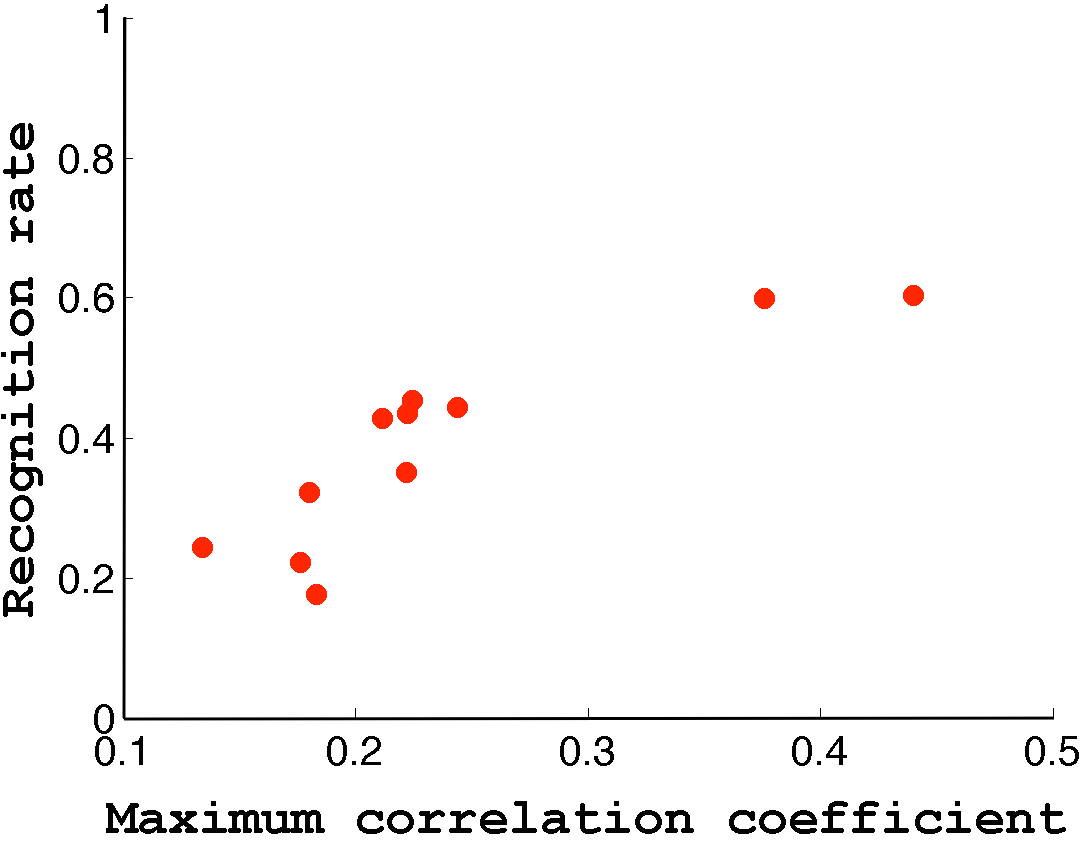
\includegraphics[width=\textwidth]{individual_accuracy_corr1.png}
                \caption{Individual accuracy - maximum of $R$}
                \label{sb1}
        \end{subfigure}
                \begin{subfigure}[b]{0.23\textwidth}
                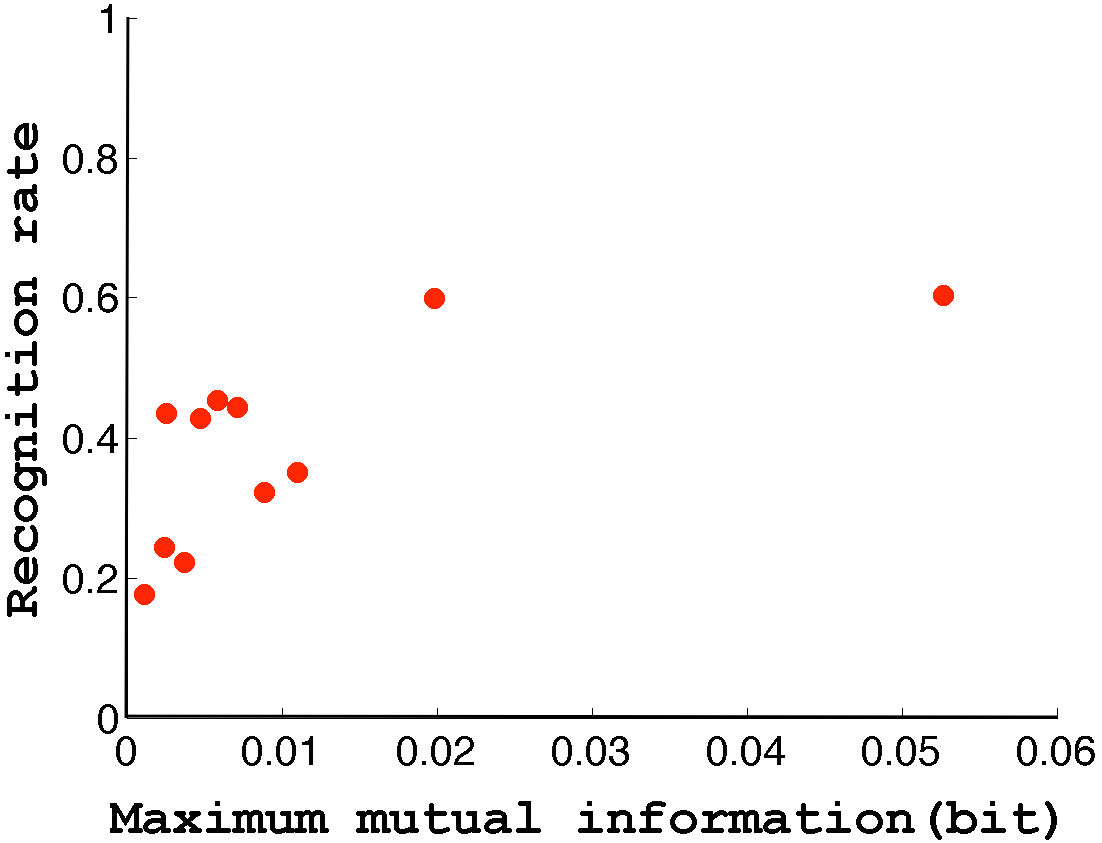
\includegraphics[width=\textwidth]{individual_accuracy_mutinf1.png}
                \caption{Individual accuracy - maximum of $I$}
                \label{sb2}
        \end{subfigure}
                \begin{subfigure}[b]{0.23\textwidth}
                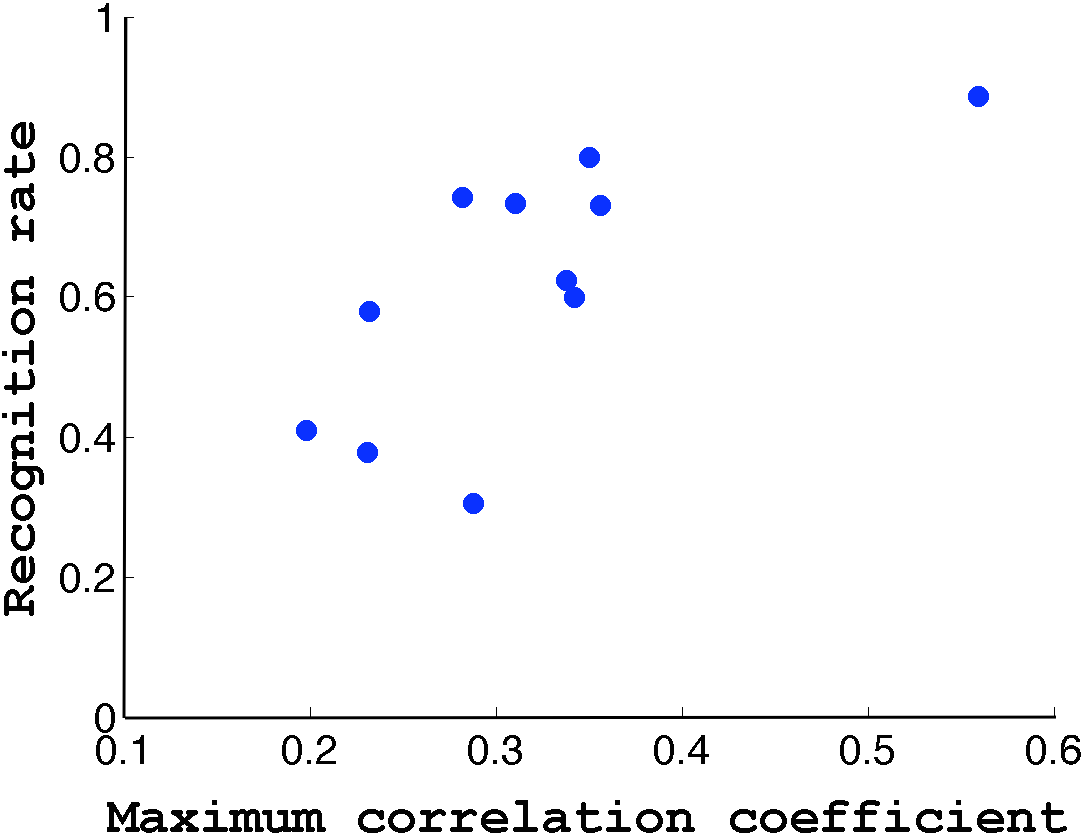
\includegraphics[width=\textwidth]{accuracy_corr1.png}
                \caption{Scene accuracy - maximum of $R$}
                \label{sb3}
        \end{subfigure}
                \begin{subfigure}[b]{0.23\textwidth}
                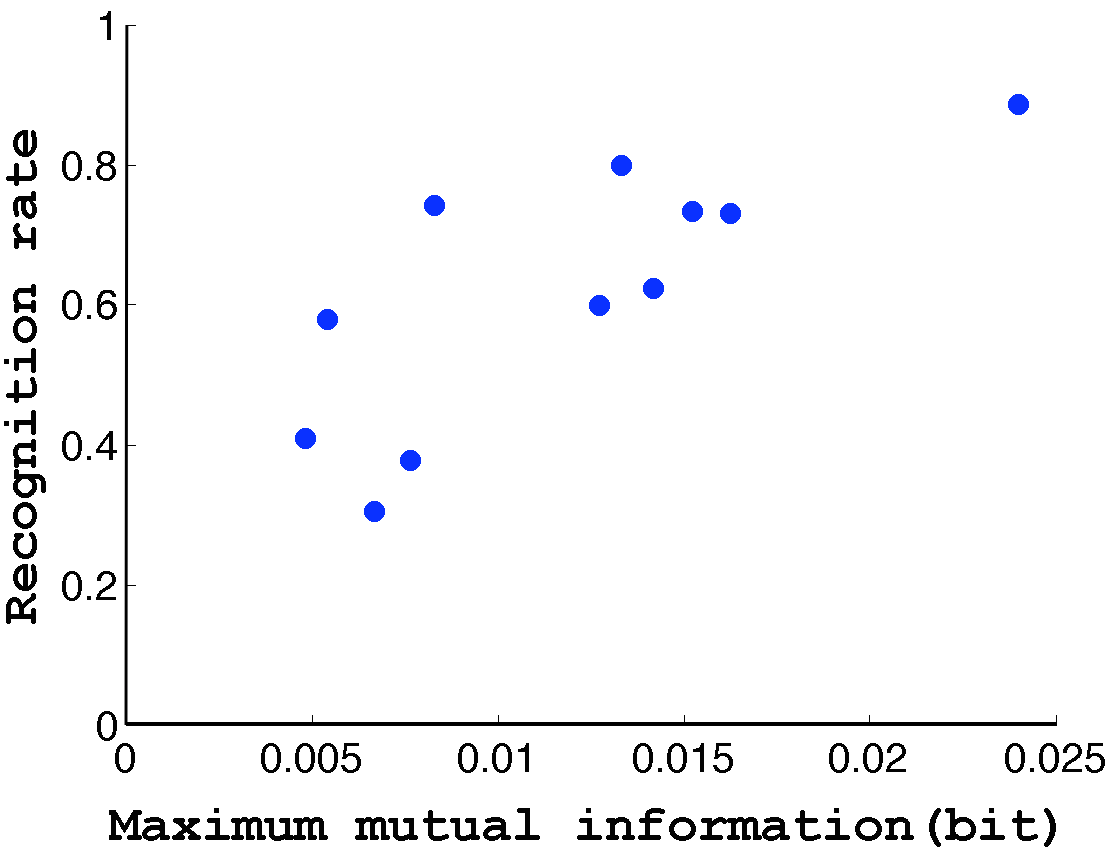
\includegraphics[width=\textwidth]{accuracy_mutinf1.png}
                \caption{Scene accuracy - maximum of $I$}
                \label{sb4}
        \end{subfigure}
\end{center}
\caption{The relationship between class-wise recognition rate and maximum of correlation $R(\textup{Pr}(l_{urban}),\textup{Pr}(l_{Imagenet}))$, class-wise recognition rate and maximum of mutual information $I(l_{urban},l_{Imagenet})$}
\label{accuracy_correlation_mutu}
\end{figure*}


%From the confusion matrix shown in Figure~\ref{confusion} for $\textup{Nets}_{SDense}$, we can observe some interesting properties of the urban tribe dataset. 8 out of 11 classes achieve higher than 60\% recognition rate, while hipster, surfer, and hiphop are three classes that are most difficult. This outcome can be explained by examining the dataset of these three groups. In the first row of Figure~\ref{images}, we take surfer group as an example. The intra-class variance of surfer group is large. Some of the scenes involve surfing activity, while others are similar to casual party.


%\emph{Formal} and \emph{goth} are two classes with highest recognition rate, being 90.5\% and 88.3\% respectively. This is intuitive: both groups have distinct characteristics, making them easier to separate from other groups. However, note that these characteristics are semantic and cannot be easily described by low-level features such as color and edge descriptors. This is illustrated in Figure~\ref{images}. Semantic property of these two classes can also be easily captured by human. This suggests the environment-people fusion features extracted in our framework shows property of group images in semantic level.  



%Figure~\ref{wrong} shows some examples of misclassified images from one training round. The top left image from country class is wrongly recognized as goth. This is probably because people in the two images are attired in black, which is the most distinct property of goth group. However, human can easily exclude this image from goth, based on the semantic features. This shows the insufficiency of the features neural network extracts. The other three images show the difficulties of the dataset. These images are ambiguous even for human, and the predicted classes by our algorithm are reasonable. 

%\begin{figure}[!t]
%\begin{center}
%\centering
%\includegraphics[width=0.8\linewidth]{images}
%\end{center}
%\caption{Random examples of three representative classes. Top: surfer, middle: formal, below: goth. Surfer group images have large variation, ranging from surfing scenes to casual party scenes. Formal and goth group images are both distinctive for people's apparel.}
%\label{images}
%\end{figure}

%\begin{figure}[!t]
%\begin{center}
%\centering
%\includegraphics[width=0.8\linewidth]{wrong_images}
%\end{center}
%\caption{Examples of misclassified images. True classes of the images are the labels in the left, while predicted classes are in the right.}
%\label{wrong}
%\end{figure}



\section{Conclusion}
In this work, we explore the use of pre-trained deep network features for social group recognition. We propose a recognition framework which takes in both individual and global features. Our results show the success of our framework. Both visualization and numeric results show the generalization ability and semantic information of pre-trained CNN features. Our results also show the necessity of  fine-tuning in social group recognition and imply the potential usage and modification of pre-trained CNN features for other computer vision tasks. 




{\small
\bibliographystyle{ieee}
\bibliography{my_paper}
}


\end{document}
